%!TEX root = ../../main.tex
\section{Processing multiple 1D aperture scan measurements}
\label{sec:Processing multiple 1D aperture scan measurements}
In section \ref{sec:Processing aperture measurements}, measurements of the X-ray beam were described which were taken by scanning a 10$\,\mu m$ aperture across the beam horizontally and vertically through the centre of the beam.
A 2D beam profile was calculated by fitting a Gaussian function to the separate profiles and substituting those parameter values in the equation of a 2D Gaussian.
The implicit assumption made is that the beam profile is similar in every region of space, including the central slices.
This is in addition to the explicit assumption that the beam profile is Gaussian.
X-ray beam profiles can vary drastically from beamline to beamline even at the same synchrotron, so the assumptions made by the previous method are not generally applicable to all beam profiles.
Therefore, a method to generate 2D X-ray beam profiles from multiple 1D aperture scans across the X-ray beam was developed to provide a more generally applicable solution to this problem.

\subsection{Acquiring the 1D aperture scans}
\label{sub:Acquiring the 1D aperture scans}
In order to estimate the dose for the SAXS experiments described in chapter \ref{chap:Methods to assess radiation damage in SAXS}, aperture scans to obtain X-ray beam flux measurements were carried out in collaboration with Dr. Adam Round and Dr. Martha Brennich on the ESRF BM29 (SAXS) beamline.
A 100$\,\mu m$ diameter circular aperture was used to scan across the X-ray beam area and measurements were taken at 10$\,\mu m$ intervals with an OSD1-0 photodiode purchased from Optoelectronics.
The scanning was performed 6 times with the collection of 3 horizontal and 3 vertical scans (Figure~\ref{fig:Aperture scans - Beam processing chapter}).
\begin{figure}
    \centering
    \begin{subfigure}[b]{0.9\textwidth}
            \centering
            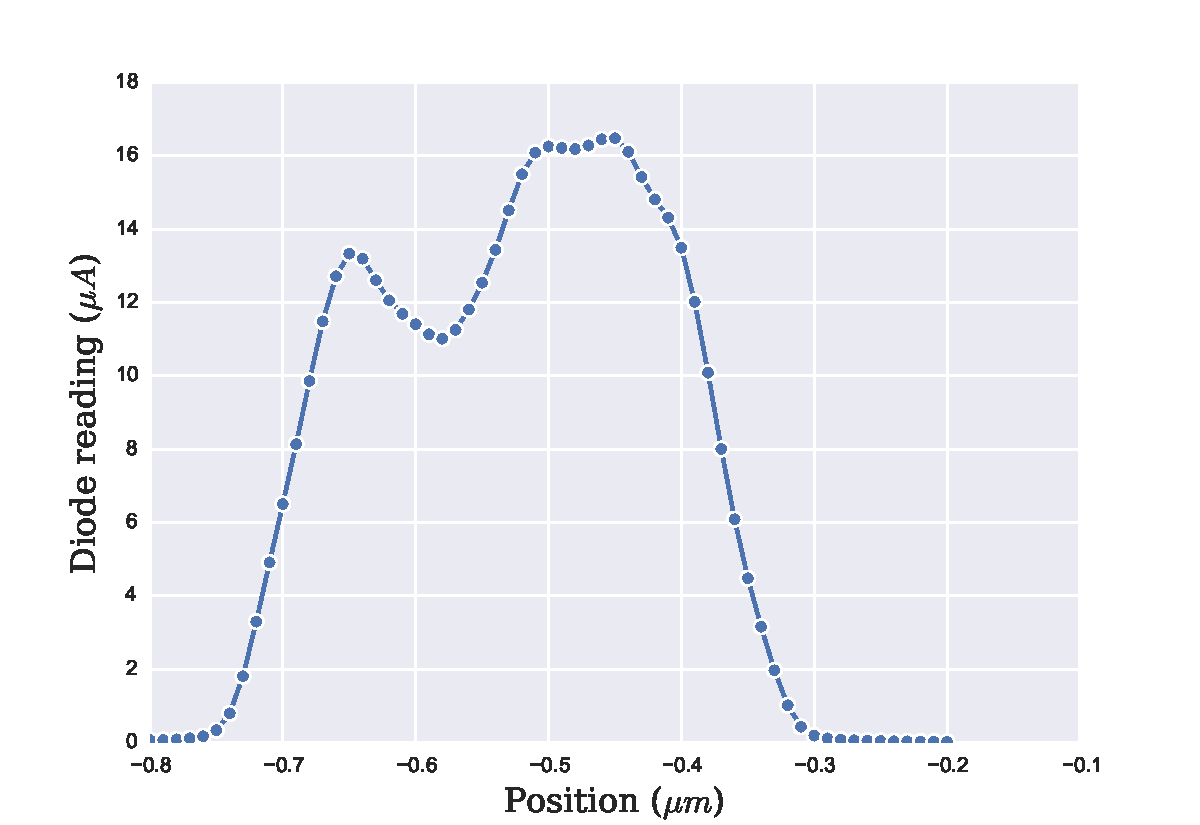
\includegraphics[width=\textwidth]{figures/beam/SAXS_vertical_aperture_scan.pdf}
            \caption{}
            \label{fig:Vertical aperture scans - Beam processing chapter}
    \end{subfigure}
    \\
    \begin{subfigure}[b]{0.9\textwidth}
            \centering
            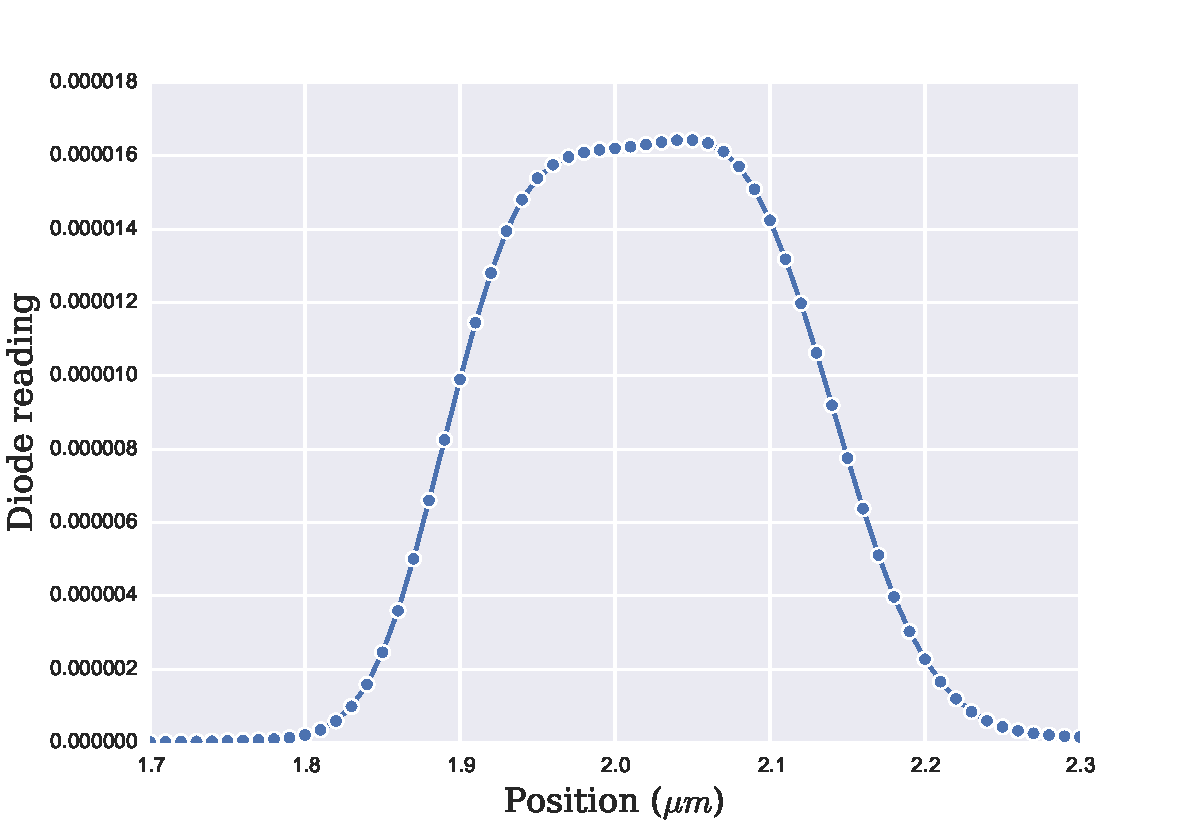
\includegraphics[width=\textwidth]{figures/beam/SAXS_horizontal_aperture_scan.pdf}
            \caption{}
            \label{fig:Horizontal aperture scans - Beam processing chapter}
    \end{subfigure}
    \caption[Diode readings from aperture scans across the beam collected at beamline BM29, ESRF.]{Diode readings from aperture scans across the beam collected at beamline BM29, ESRF, displayed in Figure~\ref{fig:SAXS beam profile}. (a) Vertical scan through the centre of the beam. (b) Horizontal scan through the centre of the beam. 4 other scans (2 vertical, 2 horizontal) were also taken at other locations across the beam.}
    \label{fig:Aperture scans - Beam processing chapter}
\end{figure}

\subsection{Creating a 2D beam profile}
\label{sub:Creating a 2D beam profile}
It is clear from the data shown in Figure~\ref{fig:Aperture scans - Beam processing chapter} that fitting a Gaussian shape will not model this beam profile well.
Instead a rectangular grid is set up with the edges of the measurement positions in Figures \ref{fig:Vertical aperture scans - Beam processing chapter} and \ref{fig:Horizontal aperture scans - Beam processing chapter} used as the boundaries of the grid.
The flux at and beyond the grid boundaries is assumed to be zero.
The diode measurements from the vertical aperture scans were placed in their corresponding positions on the grid and interpolation between these values was performed using the \verb+RectBivariateSpline+ function in SciPy package in the Python programming language \cite{jones2014scipy}.
The same procedure was performed for the data in the horizontal direction.
The results are shown in Figure~\ref{fig:Interpolation of aperture scans}.
\begin{figure}
    \centering
    \begin{subfigure}[b]{0.9\textwidth}
            \centering
            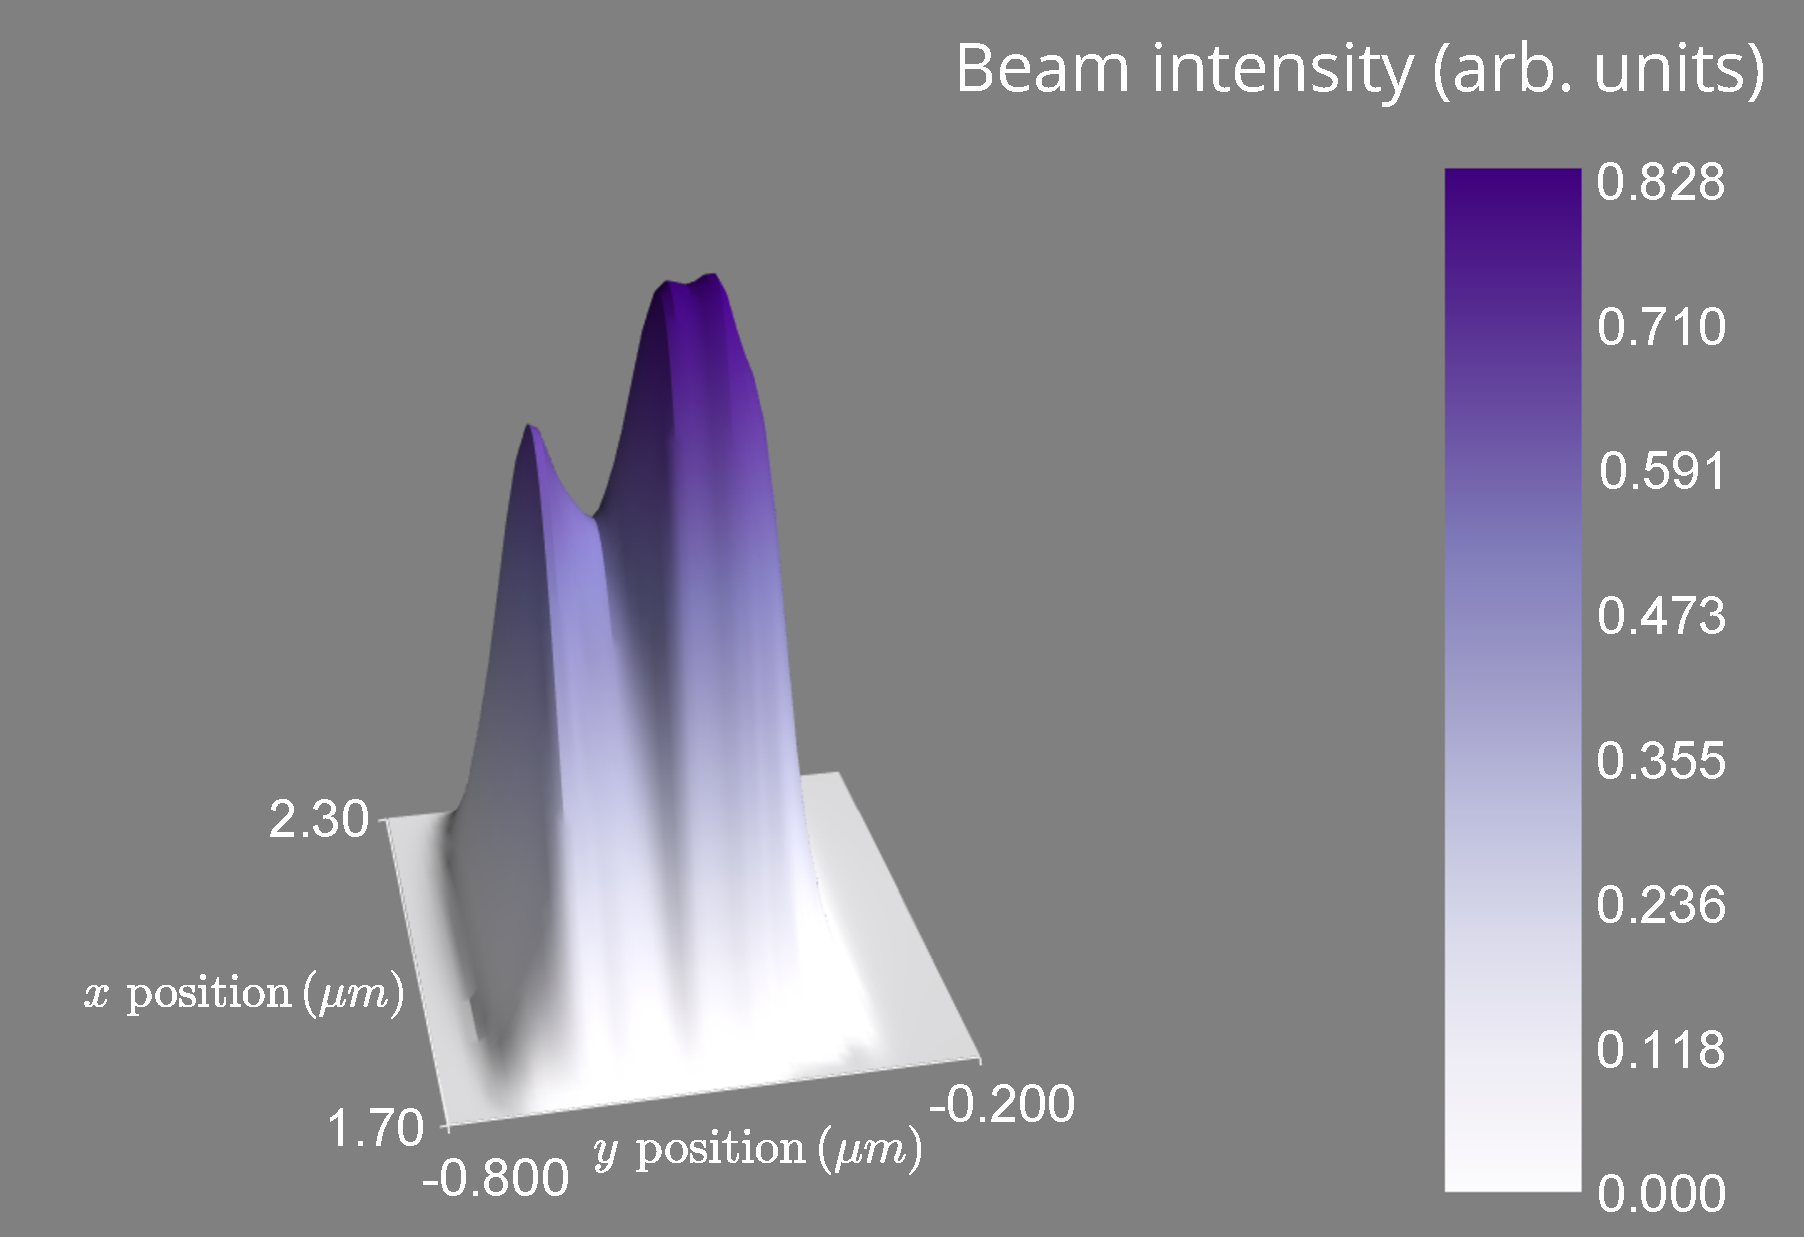
\includegraphics[width=\textwidth]{figures/beam/vert_scans_interp.pdf}
            \caption{}
            \label{fig:Interpolation of vertical aperture scans}
    \end{subfigure}
    \\
    \begin{subfigure}[b]{0.9\textwidth}
            \centering
            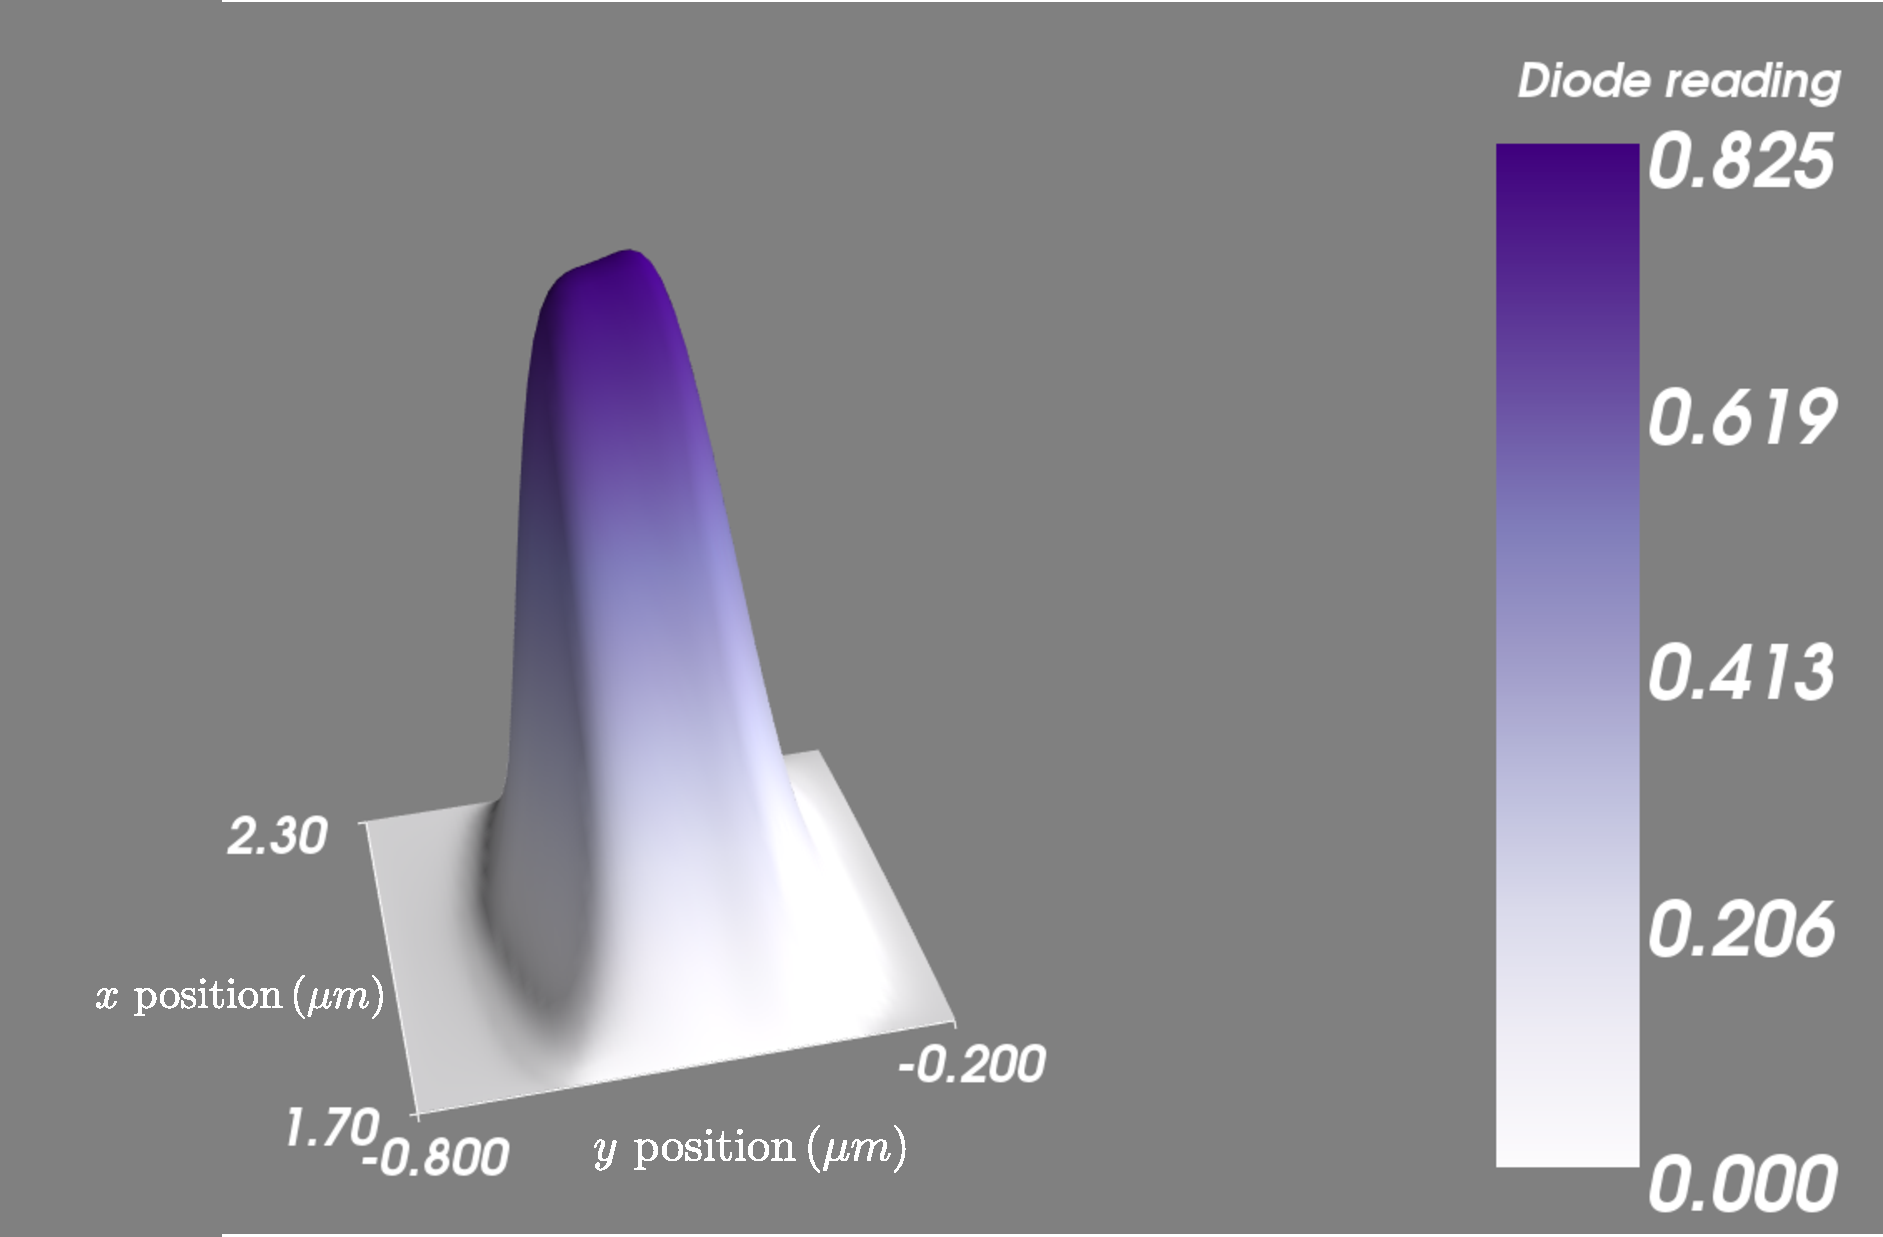
\includegraphics[width=\textwidth]{figures/beam/horiz_scans_interp.pdf}
            \caption{}
            \label{fig:Interpolation of horizontal aperture scans}
    \end{subfigure}
    \caption[Interpolation of diode readings from the aperture scans.]{Interpolation of diode readings from the aperture scans.
    (a) Interpolation of vertical scans.
    (b) Interpolation of horizontal scans.}
    \label{fig:Interpolation of aperture scans}
\end{figure}
The two interpolated arrays from Figure~\ref{fig:Interpolation of aperture scans} are then averaged to obtain the final beam profile (Figure~\ref{fig:Averaged Beam Profile} ).
\begin{figure}
    \centering
    \begin{subfigure}[b]{0.8\textwidth}
            \centering
            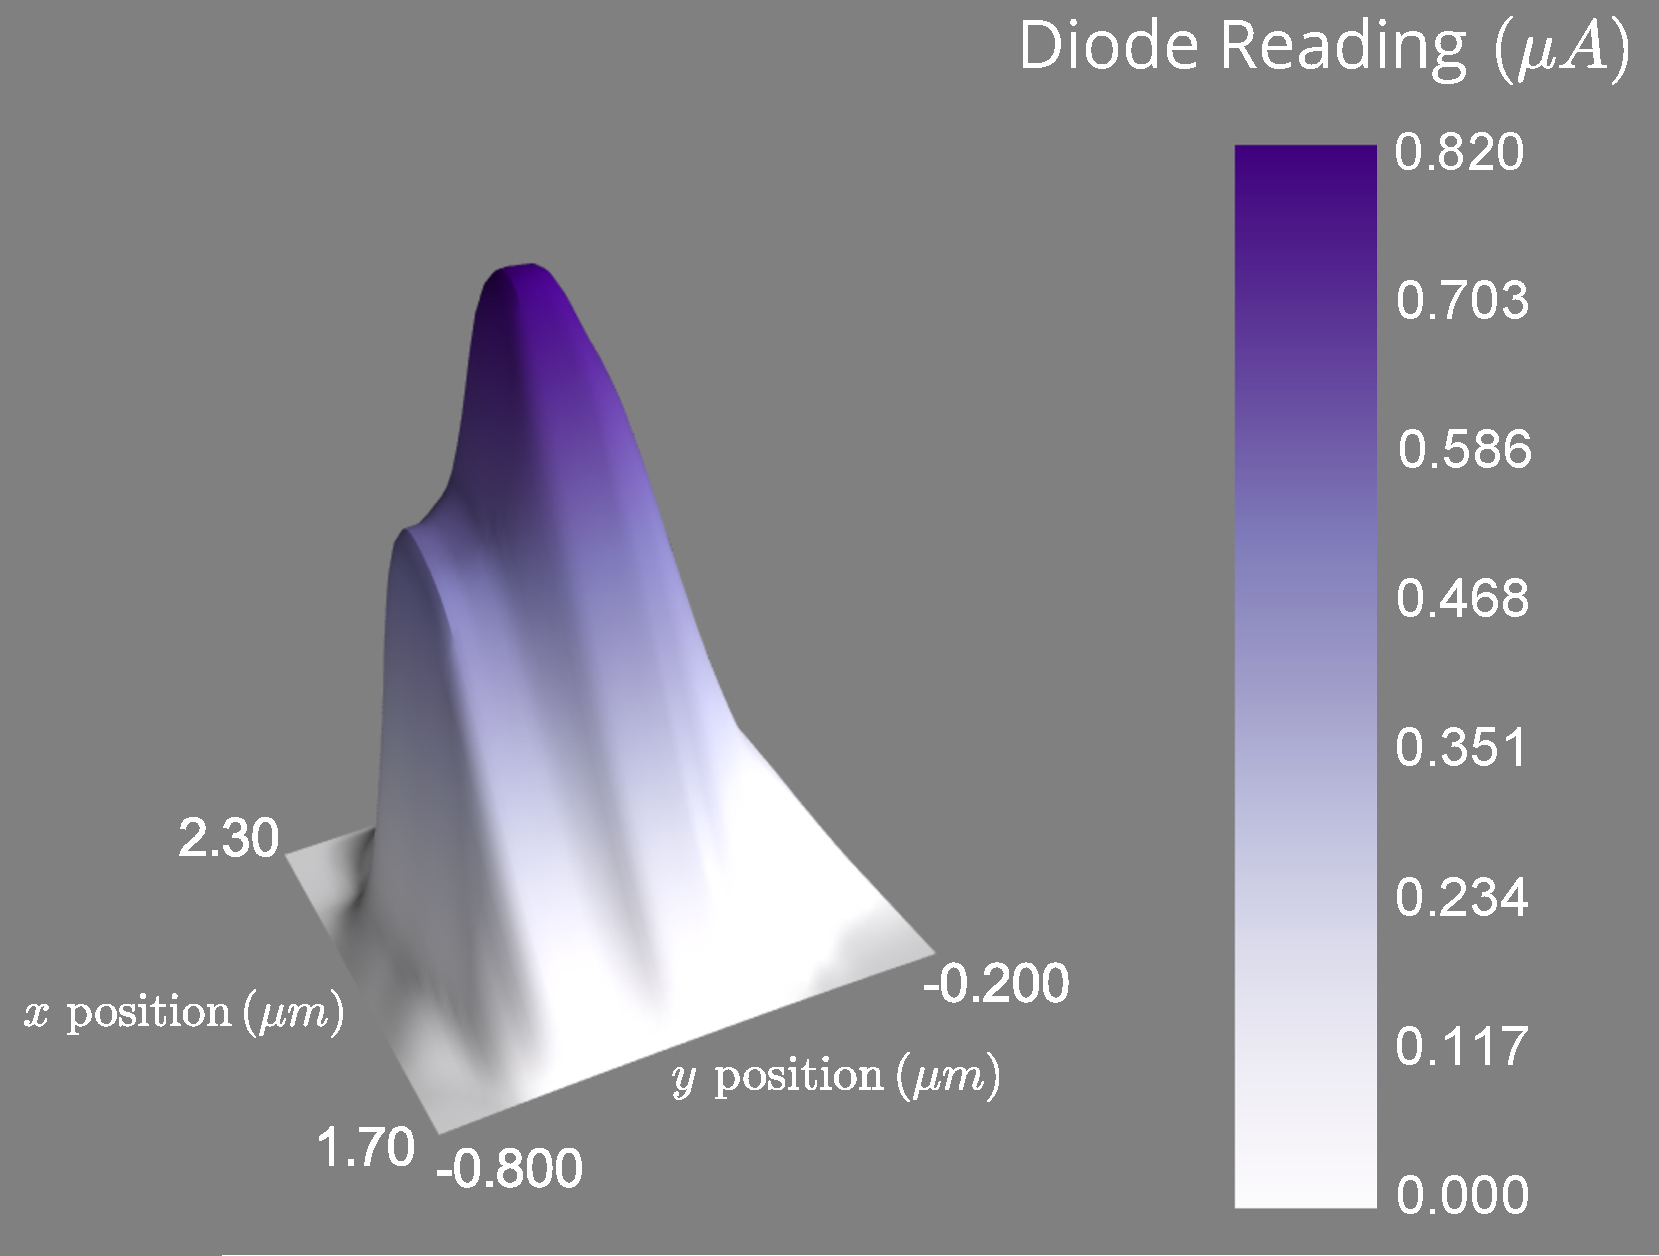
\includegraphics[width=\textwidth]{figures/beam/averaged_beam.pdf}
            \caption{}
            \label{fig:Full averaged interpolated beam}
    \end{subfigure}
    \\
    \begin{subfigure}[b]{0.75\textwidth}
            \centering
            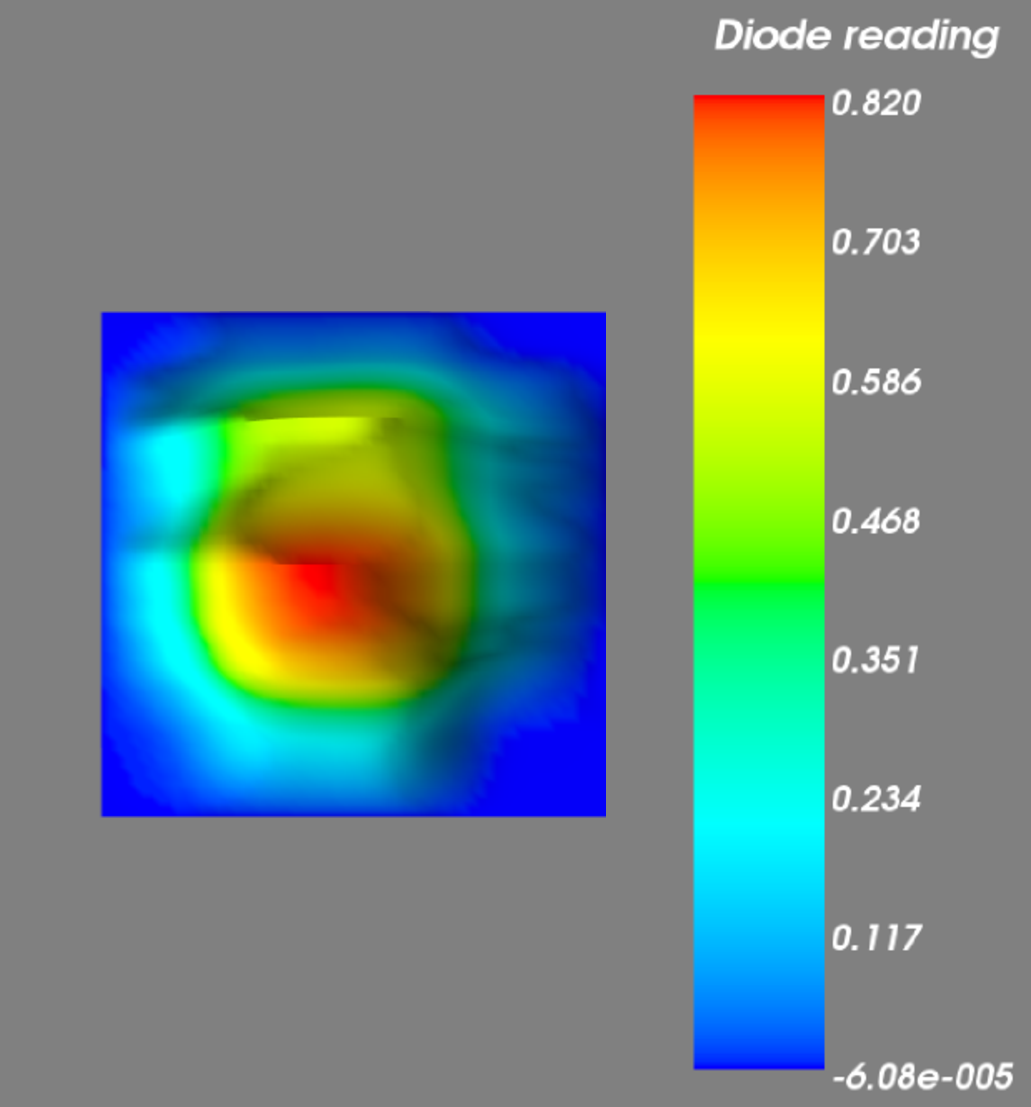
\includegraphics[width=\textwidth]{figures/beam/Overhead_beam.pdf}
            \caption{}
            \label{fig:Overhead averaged interpolated interpolated beam}
    \end{subfigure}
    \caption[Final averaged X-ray beam profile used for the SAXS experiments.]{(a) Final X-ray beam profile generated from the average of the two beams in Figure~\ref{fig:Interpolation of aperture scans}.
    (b) Overhead view with a rainbow colour scheme.}
    \label{fig:Averaged Beam Profile}
\end{figure}

The final X-ray beam profile in this case is a much truer representation of the overall beam profile than that generated by fitting a Gaussian profile.
The main reason is because the measurements are explicitly used as points on the interpolated beam profile grid as opposed to fitting a mathematical function.
Secondly, the method uses data from scans taken anywhere in the X-ray beam profile rather than just the central slices.
However, the method is not perfect because the final averaging causes a loss of some features.
Figure~\ref{fig:Interpolation of vertical aperture scans} exhibits a `valley' in the beam profile; however after averaging, the valley resembles a `shoulder' (Figure~\ref{fig:Full averaged interpolated beam}).
This could be rectified by applying a weighted averaging scheme where positions that contain measured data in one beam profile array and not the other are up weighted.
A more desirable approach would be to use an interpolation routine that could be applied to all measured data in both directions, thus avoiding the need to average at all.
It is also important to collect as many aperture scans as possible because the resulting beam profile will be more representative of the true X-ray beam profile, as then more actual values are measured.
